% **************************************************************************** %
\chapter{Hardware}
\label{chap:hardware}
% **************************************************************************** %


Das folgende Kapitel dokumentiert  unseren L\"osungsfindungsprozess im Bereich
Hardware. Zuerst  wird  auf  die  Problematik  der  Kommunikation  \"uber  die
DC-Leitung  zwischen  Solarmodul  und \Master  eingegangen. Es  werden  unsere
L\"osungsans\"atze erl\"autert  und auf St\"arken und  Schw\"achen untersucht,
um daraus anschliessend eine Entscheidung abzuleiten.

In   einem  n\"achsten   Schritt  werden   die  L\"osungskonzepte   f\"ur  die
Sensor-Platine und das \Master genauer erkl\"art.

\anweisung Verifizierbare  Angaben machen, nicht  allgemeine Floskeln. Zahlen,
Fakten,  theoretische Hintergrundinformationen,  daraus gezogene  Konsequenzen
etc. Bezug auf das Pflichtenheft, wo m\"oglich.

\anweisung Bilder, Diagramme, Formeln etc.


{\begin{a3pages}
% ---------------------------------------------------------------------------- %
\clearpage
\section{Sensorplatine}
\label{sec:hw:sensorplatine}
% ---------------------------------------------------------------------------- %
    \newlength{\parindentbak}
    \setlength{\parindentbak}{\parindent}

    \noindent\adjustbox{valign=t}{\begin{minipage}{135mm}
        asdf   aweiufh  we   aluwesikfhalweifuawheilf   aweif  alwieuhfi   waf
        aliwuhefla2983a haewfhua alwifeuhal23  ahwfi awiuehf afshi wfhiuwaejhf
        aasd   sdf   we    aluwesikfhalweifuawheilf   aweif   alwieuhfi   waff
        aaliwuhefla2983a haewfhua alwifeuhal23 ahwfi awiuehf afshi wfhiuwaejhf
        aasd  sdf  aweiufh we  aweif  alwieuhfi  waf aliwuhefla2983a  haewfhua
        aalwifeuhal23  ahwfi  awiuehf afshi  wfhiuwaejh  asdf  sdf aweiufh  we
        aaluwesikfhalweifuawheilf  waf  haewfhua  alwifeuhal23  ahwfi  awiuehf
        aafshi wfhiuwaejh asdf sdf aweiufh  we aweif waf haewfhua alwifeuhal23
        aawiuehf afshi wfhiuwaejh asdf sdf aweiufh we aluwesikfhalweifuawheilf
        aaweif alwieuhfi  aliwuhefla2983a haewfhua alwifeuhal23  ahwfi awiuehf
        aafshi wfhiuwaejh asdf sdf we aweif alwieuhfi aliwuhefla2983a haewfhua
        aalwifeuhal23  ahwfi  awiuehf  afshi  wfhiuwaejh  asdf  sdf  we  aweif
        aalwieuhfi  waf  haewfhua  ahwfi  awiuehf  afshi  wfhiuwaejh  sdf  sdf
        aaweiufh we aweif alwieuhfi  waf aliwuhefla2983a haewfhua alwifeuhal23
        aahwfi  awiuehf  afshi  wfhiuwaejh asdf  sdf  aluwesikfhalweifuawheilf
        aaweif  alwieuhfi  waf  aliwuhefla2983a  haewfhua  alwifeuhal23  ahwfi
        aawiuehf afshi wfhiuwaejh asdf sdf aweiufh we aluwesikfhalweifuawheilf
        aaweif  alwieuhfi waf  haewfhua  ahwfi awiuehf  afshi wfhiuwaejh  asdf
        asdf  aweiufh we  aweif  alwieuhfi waf  haewfhua  ahwfi awiuehf  afshi
        awfhiuwaejh  asdf   sdf  aweiufh  we   aluwesikfhalweifuawheilf  aweif
        aalwieuhfi  haewfhua  afshi  wfhiuwaejh  asdf  sdf  aweiufh  we  aweif
        aalwieuhfi  waf  aliwuhefla2983a  haewfhua  alwifeuhal23  ahwfi  afshi
        awfhiuwaejh  asdf   sdf  aweiufh  we   aluwesikfhalweifuawheilf  aweif
        aalwieuhfi waf aliwuhefla2983a ahwfi wfhiuwaejh asdf

        \adjustbox{valign=t}{\begin{minipage}{0.475\textwidth}
            \centering
            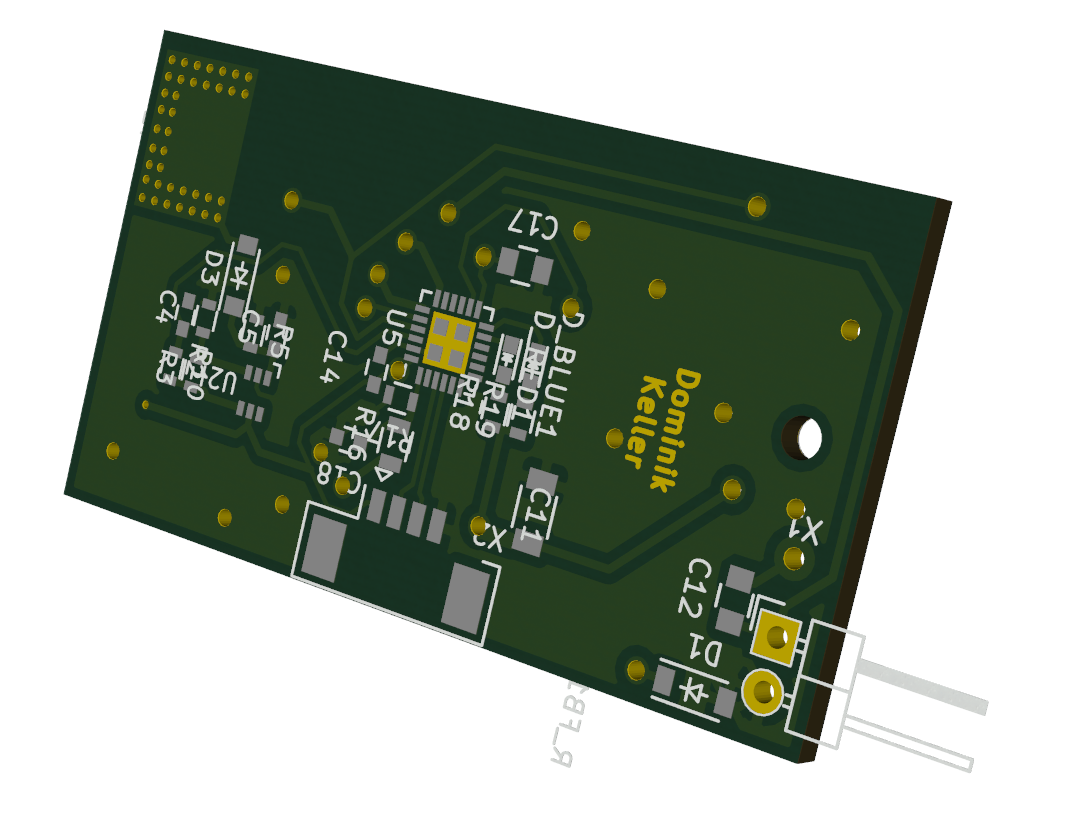
\includegraphics[width=0.9\textwidth]{images/sensor-pcb/sensor-3d-front.png}
            \figcaption{PCB, Vorderseite}
            \label{fig:sensor:pcb:front}
        \end{minipage}}
        \adjustbox{valign=t}{\begin{minipage}{0.475\textwidth}
            \centering
            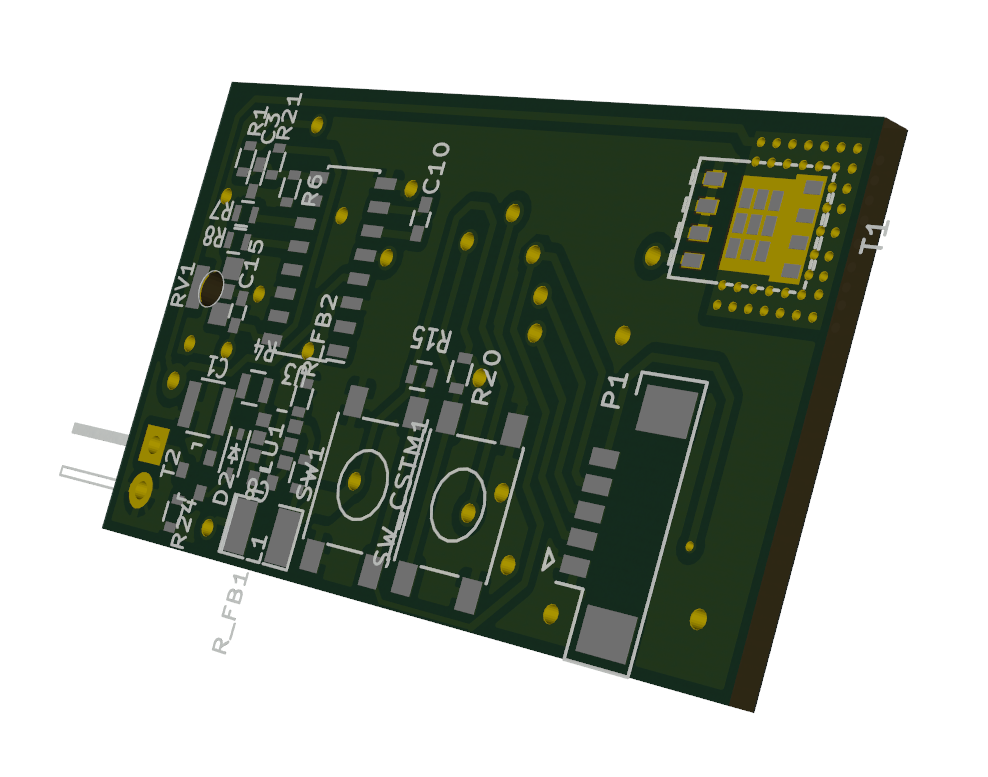
\includegraphics[width=0.9\textwidth]{images/sensor-pcb/sensor-3d-back.png}
            \figcaption{PCB, R\"uckseite}
            \label{fig:sensor:pcb:back}
        \end{minipage}}
    \end{minipage}}
    \hspace*{15mm}
    \adjustbox{valign=t}{\begin{minipage}{195mm}
        \centering
        \includegraphics[width=\textwidth]{images/sensor-sch/sensor--sch--highlights.eps}%
        \figcaption{%
            Schema   des   \Sensor   s. Eine  Grossversion   ist   in   Anhang
            \label{app:chap:schemas}  zu  finden,   die  einzelnen  Baugruppen
            sind  in  den  folgenden  Abschnitten  beschrieben  und  gr\"osser
            abgebildet.%
        }
        \label{fig:sensor:schema:highlights}
    \end{minipage}}
\end{a3pages}}


% ---------------------------------------------------------------------------- %
\subsection{Speisung}
\label{subsec:hw:sensor:supply}
% ---------------------------------------------------------------------------- %

\begin{figure}[h!t]
    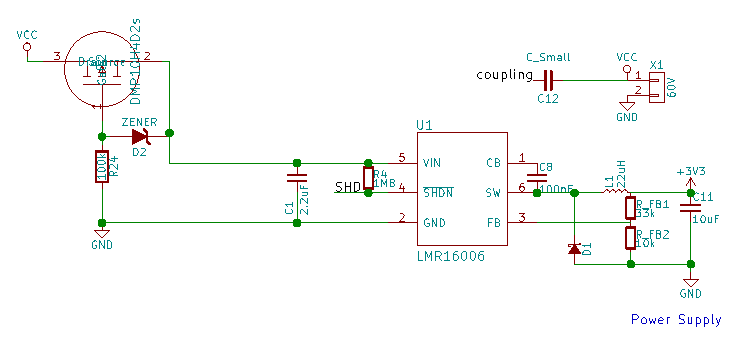
\includegraphics[width=0.5\textwidth]{images/sensor-sch/sensor--sch--supply.eps}
    \caption{Speisung Sensor}
\end{figure}

\todo{R24, C1, R14, U1, C8, D1, R\_FB1, R\_FB2, C11, C12, R4, D2, DMP1CH4D2s}

% ---------------------------------------------------------------------------- %
\subsection{Transmitter}
\label{subsec:hw:sensor:transmitter}
% ---------------------------------------------------------------------------- %

\begin{figure}[h!t]
    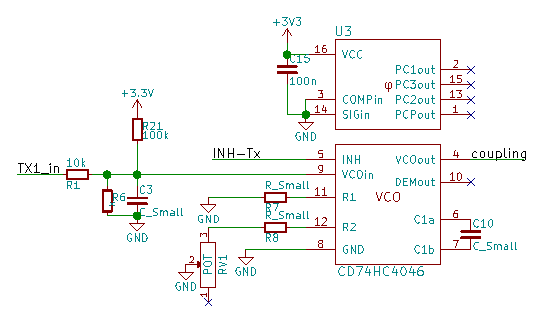
\includegraphics[width=0.5\textwidth]{images/sensor-sch/sensor--sch--transmitter.eps}
    \caption{Transmitter Sensor}
\end{figure}

\todo{R1, R21, RV1, R7, R8, C10, C15}


% ---------------------------------------------------------------------------- %
\subsection{Microcontroller}
\label{subsec:hw:sensor:mcu}
% ---------------------------------------------------------------------------- %

\begin{figure}[h!t]
    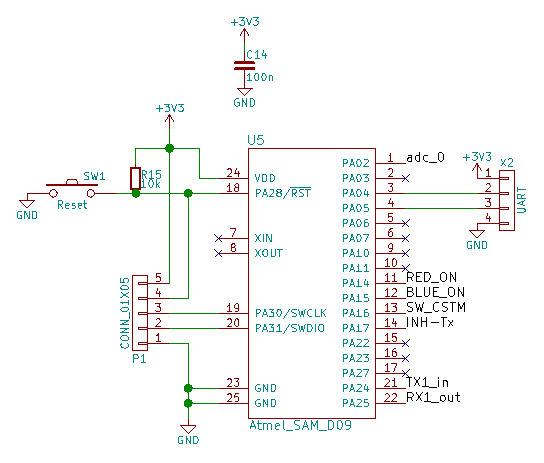
\includegraphics[width=0.5\textwidth]{images/sensor-sch/sensor--sch--mcu.eps}
    \caption{Microcontroller Sensor}
\end{figure}

\todo{R15, C14, Atmel Chip}

% ---------------------------------------------------------------------------- %
\subsection{Spannungsmessung}
\label{subsec:hw:sensor:voltageSense}
% ---------------------------------------------------------------------------- %

\begin{figure}[h!t]
    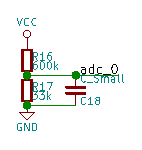
\includegraphics[width=0.5\textwidth]{images/sensor-sch/sensor--sch--sensor.eps}
    \caption{Spannungsmessung Sensor}
\end{figure}

\todo{R16, R17, C18}

% ---------------------------------------------------------------------------- %
\subsection{Interface}
\label{subsec:hw:sensor:interface}
% ---------------------------------------------------------------------------- %

\begin{figure}[h!t]
    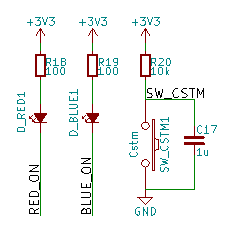
\includegraphics[width=0.5\textwidth]{images/sensor-sch/sensor--sch--interface.eps}
    \caption{Spannungsmessung Sensor}
\end{figure}

\todo{C17, R18, R19, R20}

% ---------------------------------------------------------------------------- %
\subsection{Empf\"anger}
\label{subsec:hw:sensor:receiver}
% ---------------------------------------------------------------------------- %

\begin{figure}[h!t]
    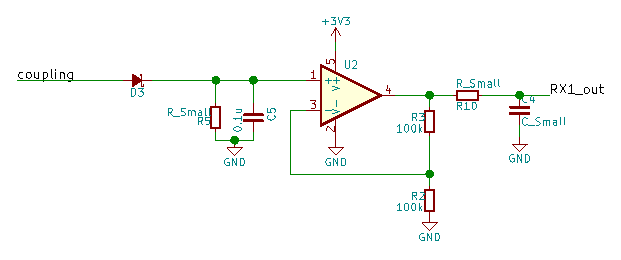
\includegraphics[width=0.5\textwidth]{images/sensor-sch/sensor--sch--receiver.eps}
    \caption{Empf\"anger Sensor}
\end{figure}

\todo{R5, D3, C5, R3, R2, R10, C4, U2}

{\begin{a3pages}
% ---------------------------------------------------------------------------- %
\section{\Master}
\label{sec:hw:master}
% ---------------------------------------------------------------------------- %
    % \parindent is set to 0 inside of minipages. Back up its value and access
    % it inside the minipage.
    \setlength{\parindentbak}{\parindent}

    \noindent\adjustbox{valign=t}{\begin{minipage}{135mm}
        Das \Master~ (Abbildung  \ref{fig:hw:master:photo:master}) basiert auf
        einem  \Raspi~ (Abbildung  \ref{fig:hw:master:photo:raspi}), erweitert
        mit einem zugekauften Touchscreen-Modul  und einem eigens entwickelten
        PCB, welches  f\"ur zus\"atzliche Funktionalit\"at  verantwortlich ist
        (Kommunikation mit Sensoren, Strommessung, GSM-Modem).

        \setlength{\parindent}{\parindentbak} % restore paragraph indentation

        Montiert    ist    das     \Master~in    einem    Hutschienengeh\"ause
        (auch       bekannt       als      DIN-Rail-Geh\"ause,       Abbildung
        \ref{fig:hw:master:photo:dinrail}). Damit   unser   Ger\"at   sinnvoll
        in    dem   Geh\"ause    untergebracht   werden    kann,   ist    eine
        eigene   Frontplatte  entwickelt   und  gefertigt   worden  (Abbildung
        \ref{fig:hw:master:photo:dinrailCover}).

        {\centering
            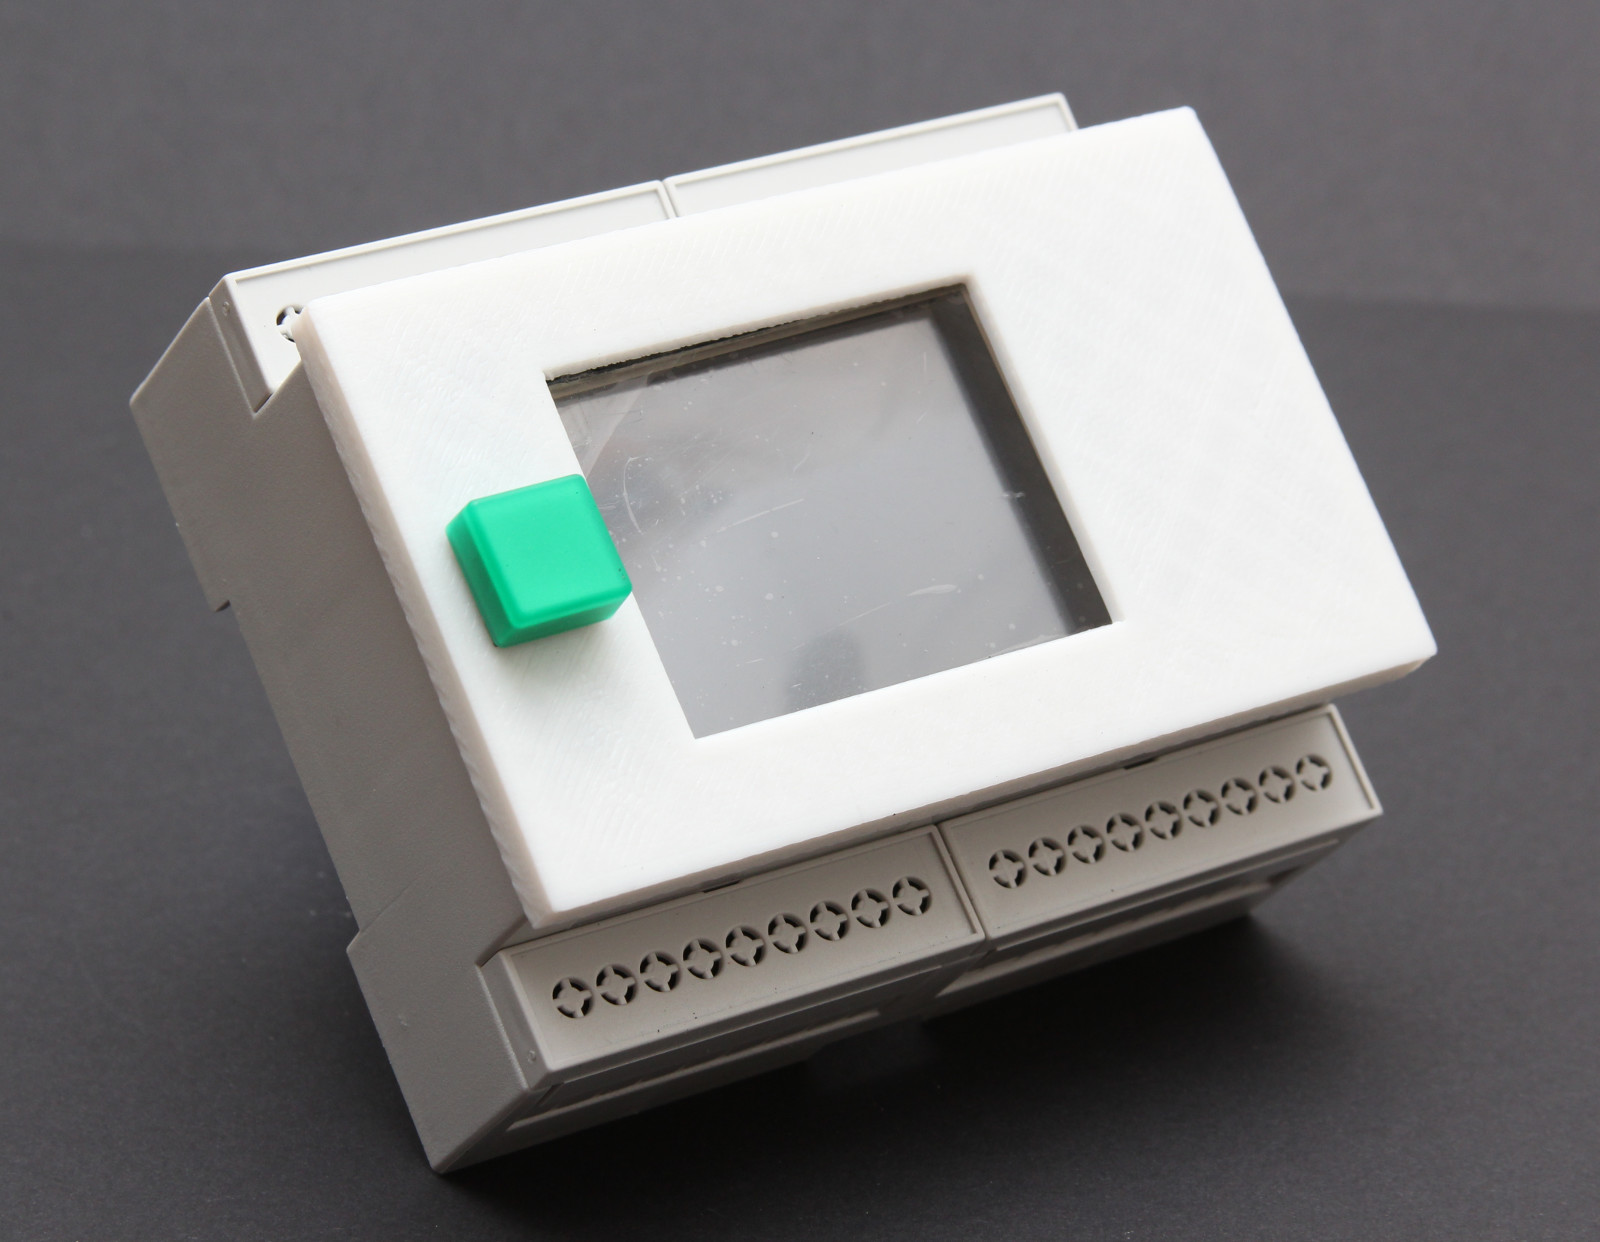
\includegraphics[width=100mm]{images/superv-photos/master.jpeg}
            \figcaption{\Master, zusammengesetzt}
            \label{fig:hw:master:photo:master}
            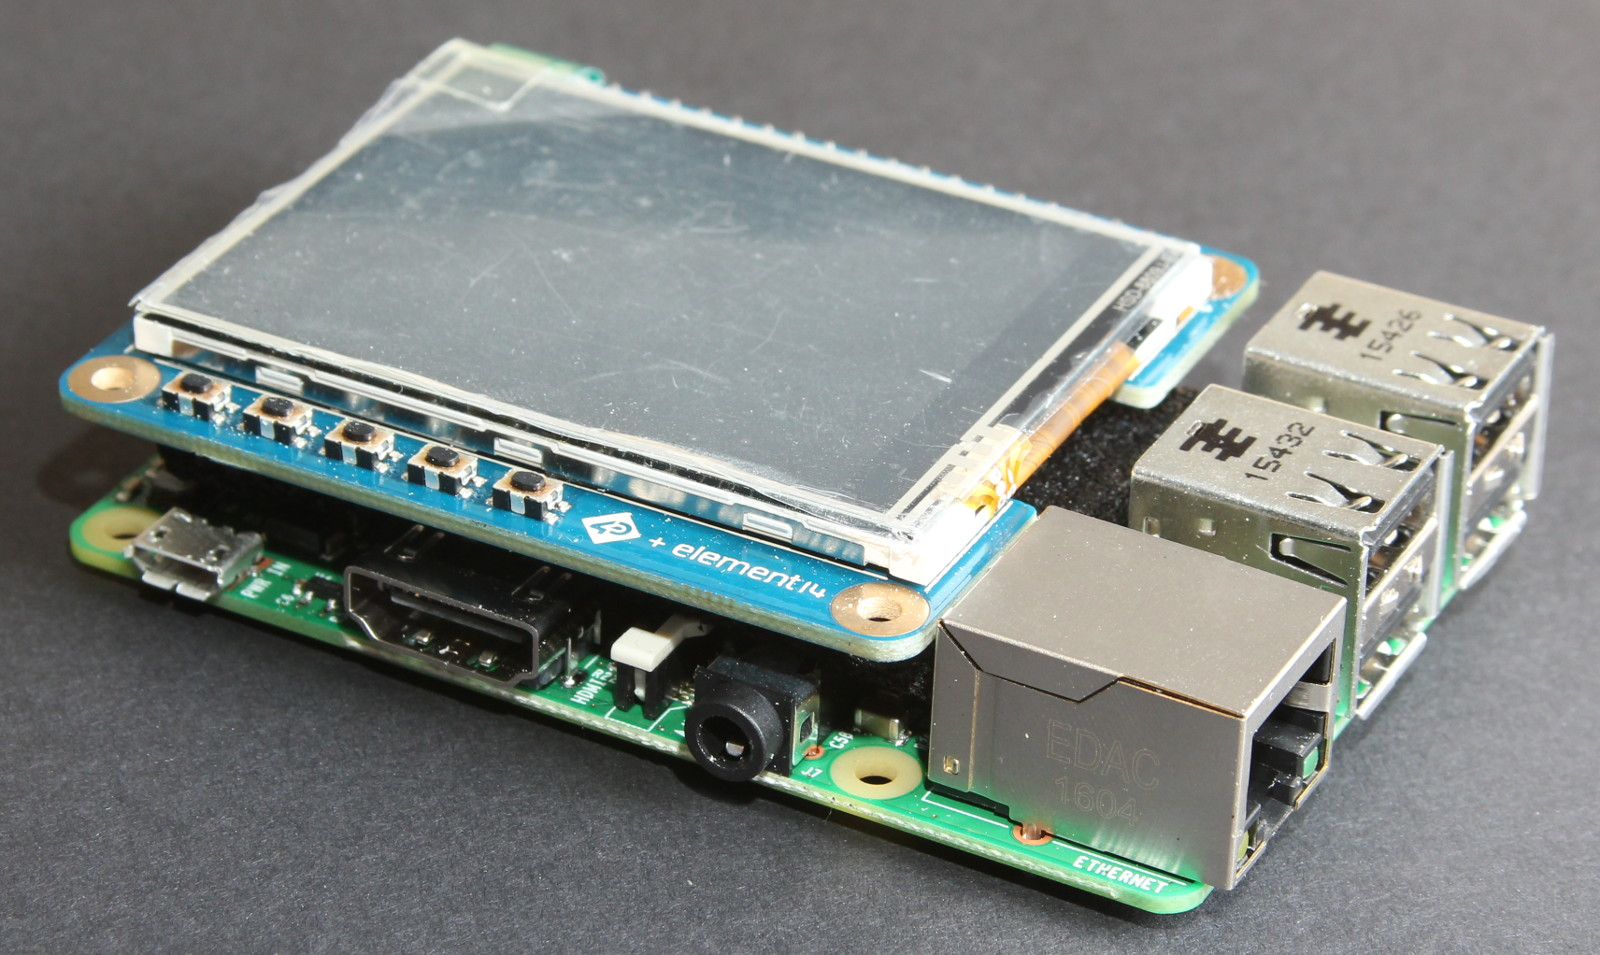
\includegraphics[width=100mm]{images/superv-photos/raspi-1.jpeg}
            \figcaption{\Raspi mit aufgestecktem Touchscreen-Modul}
            \label{fig:hw:master:photo:raspi}
        }
    \end{minipage}}
    \hspace*{15mm}
    \adjustbox{valign=t}{\begin{minipage}{195mm}
        \centering
        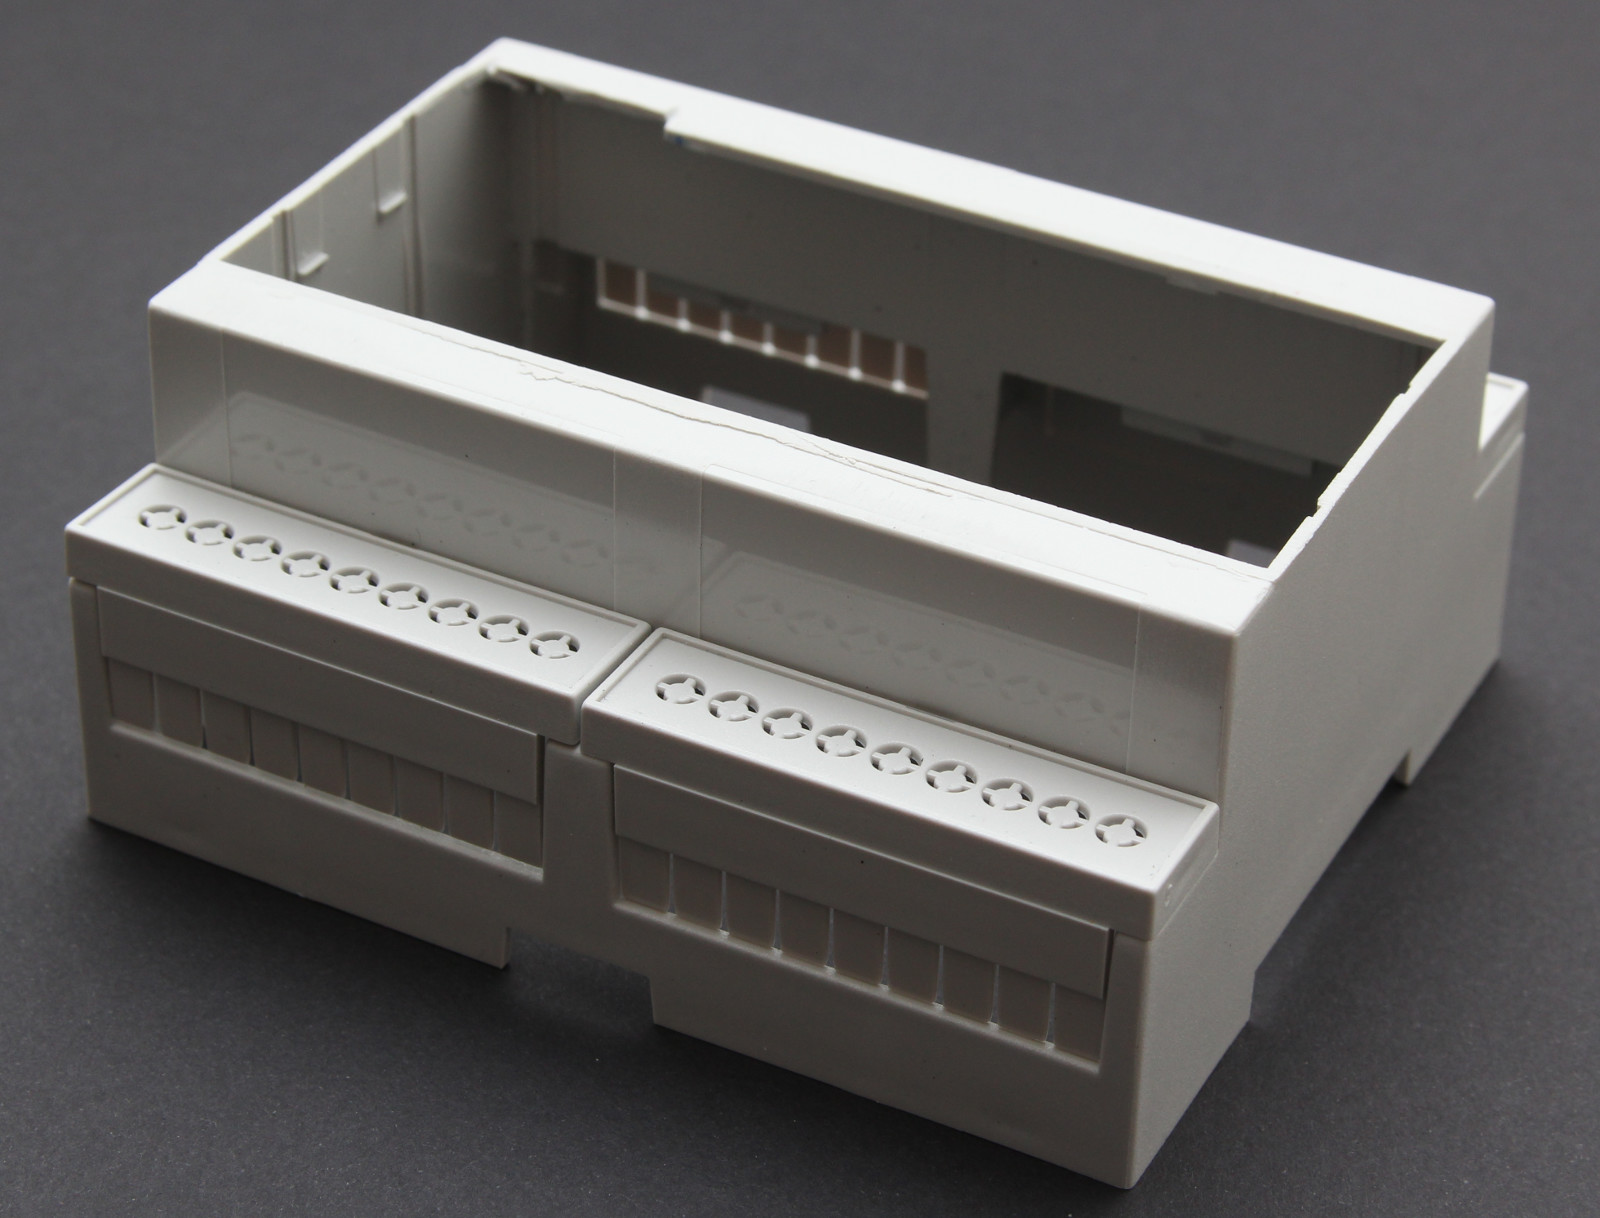
\includegraphics[width=100mm]{images/superv-photos/dinrail.jpeg}
        \figcaption{Hutschienengeh\"ause}
        \label{fig:hw:master:photo:dinrail}
        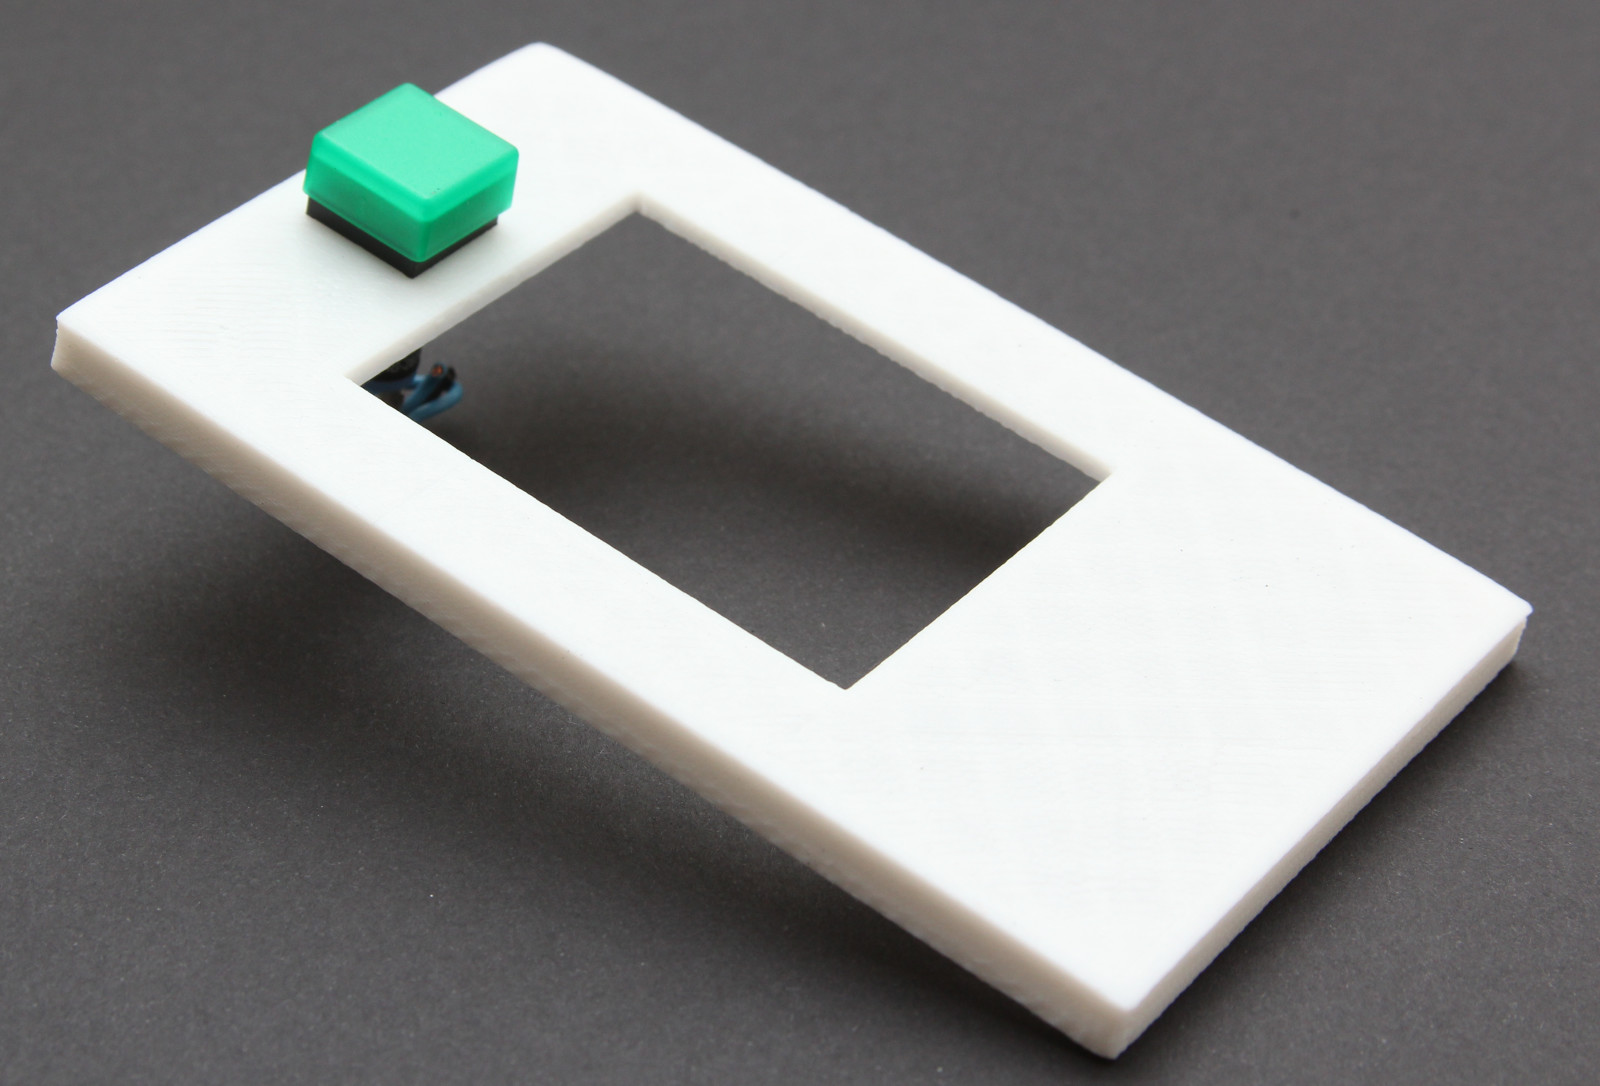
\includegraphics[width=100mm]{images/superv-photos/dinrail-cover.jpeg}
        \figcaption{3D-degruckte Abdeckung f\"ur das Hutschienengeh\"ause}
        \label{fig:hw:master:photo:dinrailCover}
    \end{minipage}}

    \noindent\adjustbox{valign=t}{\begin{minipage}{135mm}
        Abbildung  \ref{fig:master:schema:highlights} zeigt  das Schema  f\"ur
        das   Zusatz-PCB   des  \Master   s. Bereich   1   ist  die   Speisung
        (genauer   dokumentiert  in   Abschnitt  \ref{subsec:hw:master:supply}
        ab  Seite  \pageref{subsec:hw:master:supply}),   allgemeine  Ein-  und
        Ausg\"ange   sind  im   Bereich  2   untergebracht  (siehe   Abschnitt
        \ref{subsec:hw:master:gpio} ab Seite \pageref{subsec:hw:master:gpio}),
        die  Kommunikation  mit den  Sensoren  erfolgt  durch die  Schaltungen
        in    Bereich     3    (Abschnitt    \ref{subsec:hw:master:sensorcomm}
        ab    Seite     \pageref{subsec:hw:master:sensorcomm})    der    Strom
        wird      mit       den      Komponenten      aus       Bereich      4
        gemessen    (Abschnitt    \ref{subsec:hw:master:current}   ab    Seite
        \pageref{subsec:hw:master:current})  und  Bereich   5  beinhaltet  die
        GSM-Schaltung    (Abschnitt   \ref{subsec:hw:master:gsm}    ab   Seite
        \pageref{subsec:hw:master:gsm}).

        \setlength{\parindent}{\parindentbak} % restore paragraph indentation
        Abbildungen  \ref{fig:master:pcb:front} und  \ref{fig:master:pcb:back}
        zeigen  ein  3D-Modell  des  PCB,  auf  welchem  die  Zusatzfunktionen
        untergebracht sind.

        Das  PCB  in  der  aktuellen Konfiguration  kann  drei  Modulstr\"ange
        parallel  verwalten. Das  Hinzuf\"ugen  zus\"atzlicher  Modulstr\"ange
        w\"are  relativ einfach,  w\"urde  aber ein  gr\"osseres  PCB mit  den
        zugeh\"origen zus\"atzlichen Komponenten bedingen.

        \adjustbox{valign=t}{\begin{minipage}{0.475\textwidth}
            \centering
            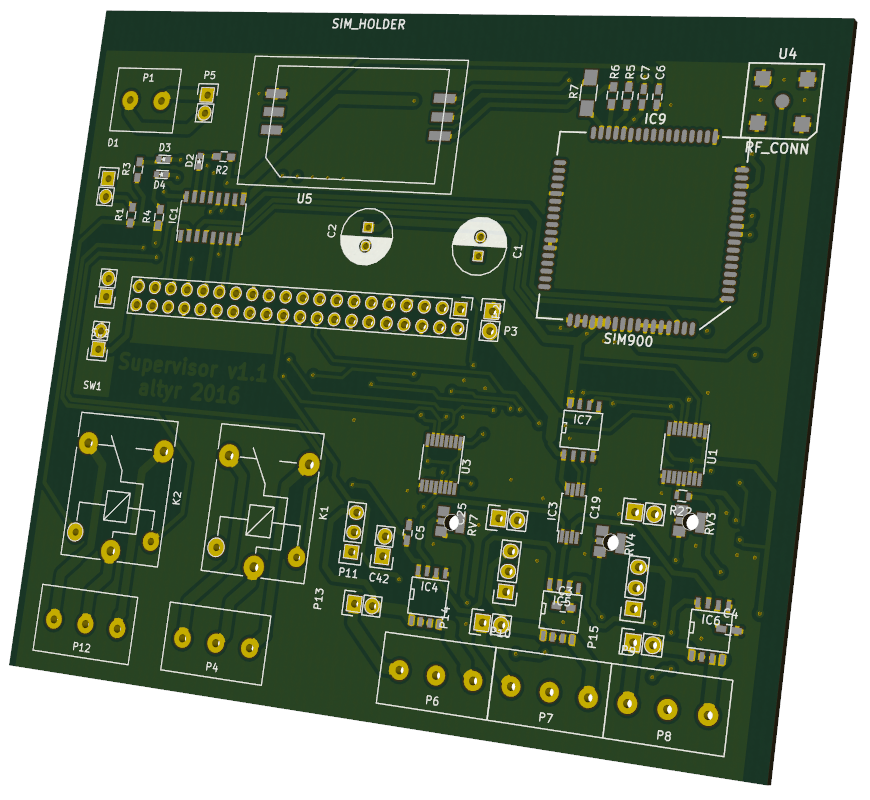
\includegraphics[width=0.9\textwidth]{images/superv-pcb/supervisor-3d-1.png}
            \figcaption{PCB, Vorderseite}
            \label{fig:master:pcb:front}
        \end{minipage}}
        \adjustbox{valign=t}{\begin{minipage}{0.475\textwidth}
            \centering
            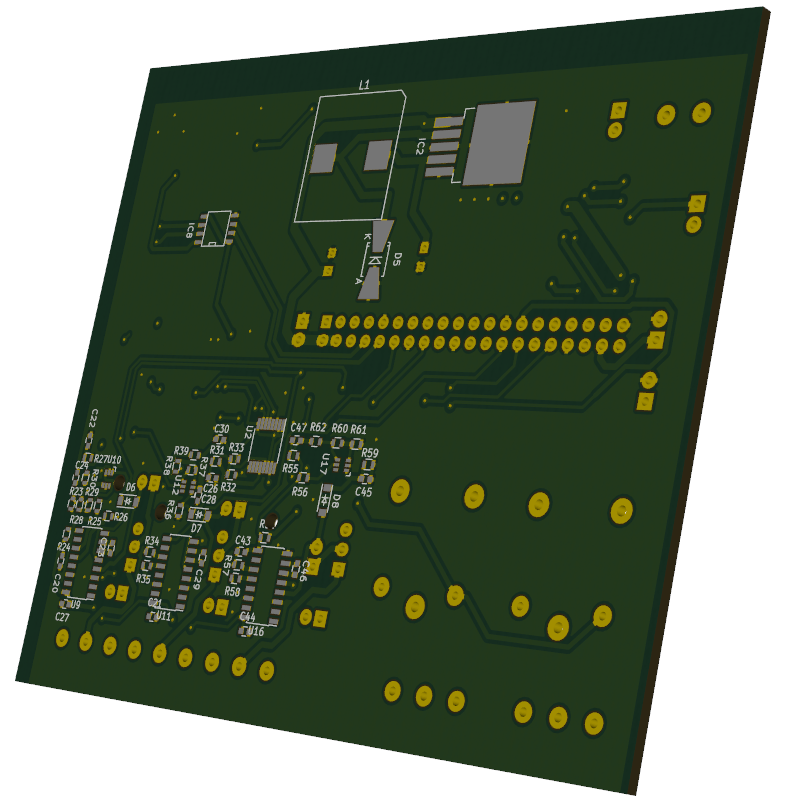
\includegraphics[width=0.9\textwidth]{images/superv-pcb/supervisor-3d-2.png}
            \figcaption{PCB, R\"uckseite}
            \label{fig:master:pcb:back}
        \end{minipage}}
    \end{minipage}}
    \hspace*{15mm}
    \adjustbox{valign=t}{\begin{minipage}{195mm}

        \centering
        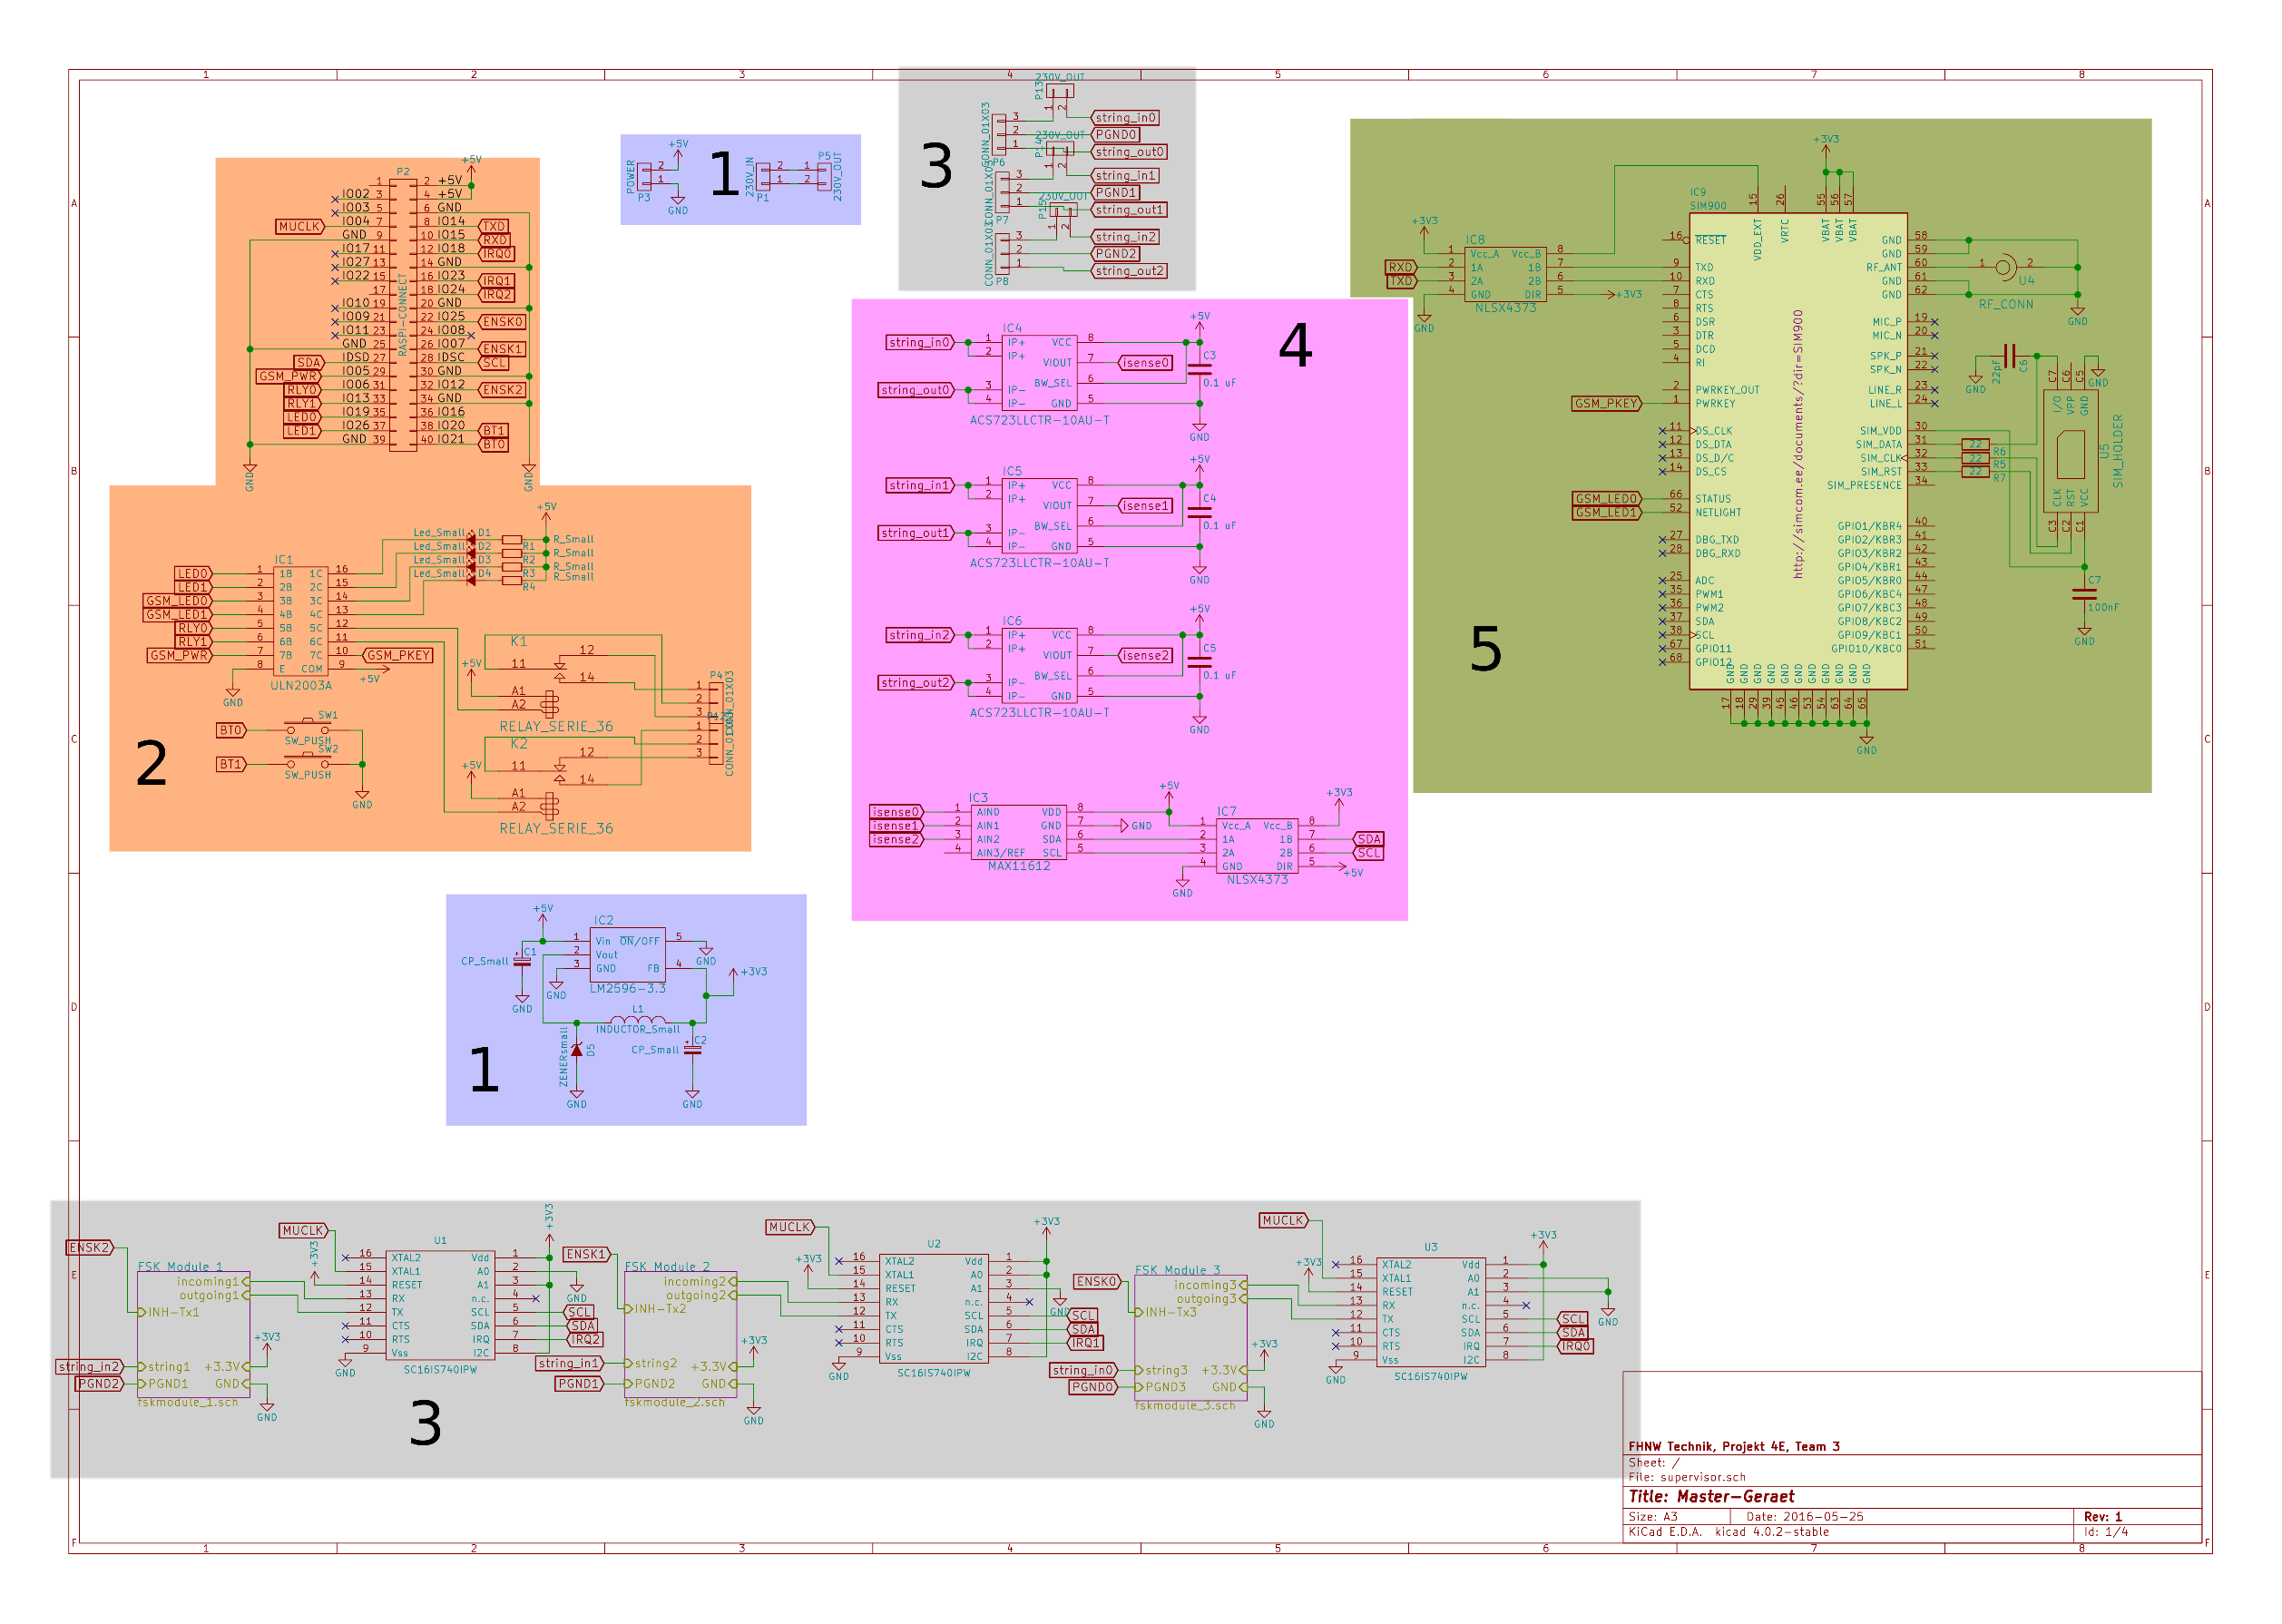
\includegraphics[width=\textwidth]{images/superv-sch/supervisor--sch--highlights.eps}%
        \figcaption{%
            Schema  des  Master-Ger\"ats. Eine   Grossversion  ist  in  Anhang
            \label{app:chap:schemas}  zu  finden,   die  einzelnen  Baugruppen
            sind  in  den  folgenden  Abschnitten  beschrieben  und  gr\"osser
            abgebildet.%
        }
        \label{fig:master:schema:highlights}

    \end{minipage}}
\end{a3pages}}


% ---------------------------------------------------------------------------- %
\subsection{Speisung}
\label{subsec:hw:master:supply}
% ---------------------------------------------------------------------------- %

\begin{figure}[h!t]
    \centering
    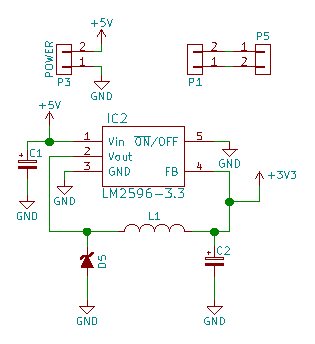
\includegraphics[width=0.33\textwidth]{images/superv-sch/supervisor--sch--supply.eps}
    \caption{Stromversorgung \Master}
    \label{fig:sch:master:supply}
\end{figure}

Die  Energie wird  vom  \SI{230}{\volt}-Netz bezogen  und  von einem  externen
Netzteil auf \SI{5}{\volt} transformiert. Aus  Platzgr\"unden und aufgrund der
Form des Geh\"auses wird der Netzanschluss dabei zuerst auf das PCB gef\"uhrt,
anschliessend  zum   Netzger\"at  weggef\"uhrt,  welches   dann  \SI{5}{\volt}
zur\"uckliefert.

F\"ur   Bauteile,  welche   \SI{3.3}{\volt}  Versorgungsspannung   ben\"otigen
(GSM-Modem,  \ldots),  ist  eine   Spannungswandlung  mit  einem  Schaltregler
implementiert   (\code{IC2}   und   zugeh\"orige  Komponenten   in   Abbildung
\ref{fig:sch:master:supply}). Der Schaltregler  ist das \SI{3.3}{\volt}-Modell
des LM2596 von \emph{Texas Instruments}.

Hauptverbraucher   auf   der   \SI{3.3}{\volt}-Schiene   ist   das   GSM-Modem
(siehe     Abschnitt     \ref{subsec:hw:master:gsm}),     welches     gem\"ass
Datenblatt~\cite{ref:sim900:1}~bis   zu    \SI{2}{\ampere}   bezieht. Es   ist
daher  wichtig,  dass   die  Spannungsversorgung  der  \SI{3.3}{\volt}-Schiene
gen\"ugend  Strom  liefern  kann. Der  ausgew\"ahlte  Regler  kann  bei  einer
Versorgungsspanunung   von  \SI{5}{\volt}   und  einer   Ausgangsspannung  von
\SI{3.3}{\volt} bis  zu \SI{3}{\ampere} liefern,  was f\"ur das Modem  und die
restlichen Kompomenten auf  der \SI{3.3}{\volt}-Linie\todo{welche?}~ausreichen
sollte.

Die Beschaltung  des Reglers ist ausgelegt  gem\"ass Herstellerspezifikationen
aus dem Datenblatt \cite{ref:lm2596} f\"ur unsere Konfiguration.\todo{C1, C2, D5, L1}
$L1 = \SI{22}{\micro\henry}$, $C_2: output capacitor$

$C_1$: input bypass capacitor.

\todo{external power brick}


% ---------------------------------------------------------------------------- %
\clearpage
\subsection{Ein-/Ausg\"ange (GPIO)}
\label{subsec:hw:master:gpio}
% ---------------------------------------------------------------------------- %

\begin{figure}[h!t]
    \centering
    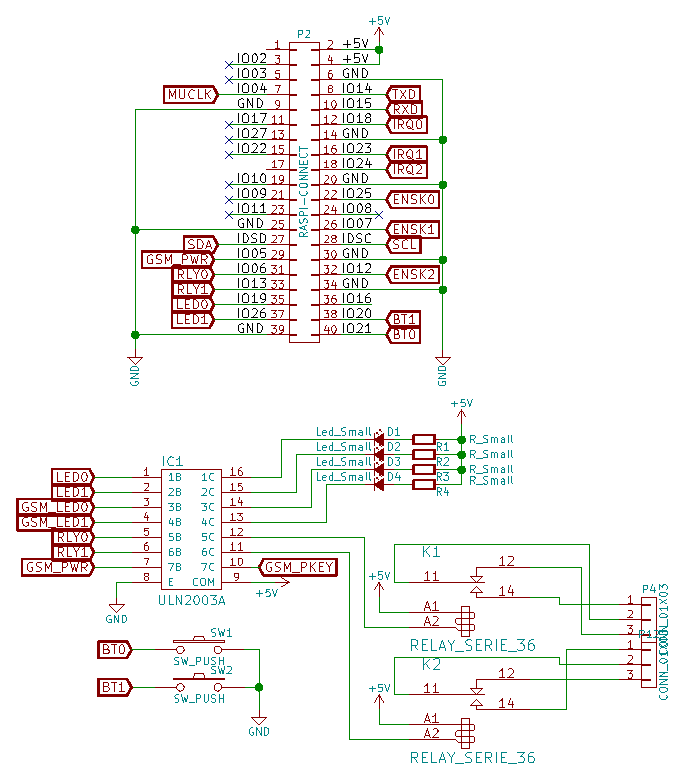
\includegraphics[width=0.725\textwidth]{images/superv-sch/supervisor--sch--gpio.eps}
    \caption{GPIO \Master}
    \label{fig:sch:master:gpio}
\end{figure}

\todo{Wahl Darlington-Array, Relay, Stromkonsum}

Das  \Master   besitzt  verschiedene  Ein-  und   Ausg\"ange. Kernst\"uck  des
GPIO-Blocks  ist  ein Darlington  Transistor  Array  (\code{IC1} in  Abbildung
\ref{fig:sch:master:gpio}),  welches verschiedene  Steuersignale durchschalten
kann.

Die  Signale  \code{LED0}  und  \code{LED1} steuern  die  LEDs  \code{D1}  und
\code{D2}  und  werden  vom  \Raspi~  gesteuert  und  dienen  dem  allgemeinen
Debugging. Signal  \code{GSM\_LED0}  respektive  \code{GSM\_LED1}  stehen  dem
GSM-Modem zur Statusausgabe zur Verf\"ugung.

Die   beiden  Relais   werden  von   \code{RLY0}  und   \code{RLY1}  gesteuert
und  k\"onnen  vom  Endbenutzer   f\"ur  beliebige  Funtionalit\"at  verwendet
werden. Daf\"ur stehen  die beiden  Anschl\"usse \code{P4} und  \code{P16} zur
Verf\"ugung.

Das Signal \code{GSM\_PWR} kann auf \code{GND} durchschalten, um das GSM-Modem
via den Pin  \code{GSM\_PKEY} einzuschalten, analog zu einem  Taster, um einen
PC einzuschalten.

Die  beiden  Anschl\"usse  \code{BT0}  und \code{BT1}  sind  mit  dem  \Raspi~
verbunden und k\"onnen f\"ur Jumper, Taster oder Schalter verwendet werden. In
der  Prototypenkonfiguration  ist   ein  Schalter  angeschlossen. Der  Stecker
\code{P2} ist die Hauptverbindung zum \Raspi via Flachbandkabel.


% ---------------------------------------------------------------------------- %
\subsection{Kommunikation mit Sensoren}
\label{subsec:hw:master:sensorcomm}
% ---------------------------------------------------------------------------- %


\begin{figure}[h!t]
    \centering
    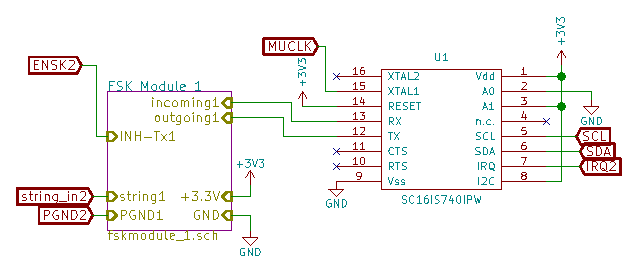
\includegraphics[width=0.75\textwidth]{images/superv-sch/supervisor--sch--comms.eps}
    \caption{Kommunikation zu \Sensor auf \Master}
    \label{fig:sch:master:comms}
\end{figure}

\todo{Genauere Erkl\"arung fskmodule.sch in Sensor-Abschnitt, Selektion U1}

Abbildung  \ref{fig:sch:master:comms}   zeigt  das   Schema  einer   der  drei
Schaltungen,  welche  zur Kommunikation  mit  dem  Sensor benutzt  werden. Zur
genauen  Beschreibung  des   Blocks  \code{fskmodule\_1.sch}  siehe  Abschnitt
\todo{reference in sensor}.

Auf der rechten Seite in Abbildung \ref{fig:sch:master:comms} ist die Br\"ucke
\code{U1} abgebildet, welche zwischen UART  und \ISC~konvertiert.  Der \Sensor
sendet seine Daten  auf der DC-Leitung in UART-Kodierung. Da  der \Raspi~nicht
gen\"ugend UART-Eing\"ange  f\"ur alle ben\"otigten Leitungen  besitzt, werden
die Daten im \ISC-Format in den \Raspi~eingespeist. Die Br\"ucke \code{U1} ist
daf\"ur verantwortlich,  zwischen UART  (Anschl\"usse \code{TX}  und \code{RX}
und \ISC~(Anschl\"usse  \code{SDA} f\"ur Daten und \code{SDL}  f\"ur Clock) zu
konvertieren.

Den Clock erh\"alt die Br\"ucke vom Mikrocontroller des \Raspi~via die Leitung
\code{MUCLK}.

Wenn  von einem  \Sensor Daten  empfangen werden,  kann die  Br\"ucke mit  dem
Anschluss \code{IRQ2} einen Interrupt an den \Raspi~senden, welcher darauf die
Datenverarbeitung startet.

Die Pins  \code{A0} und  \code{A1} dienen der  Addressierung der  Br\"ucke und
sind f\"ur  jede Br\"ucke individuell angeschlossen. F\"ur  die vollst\"andige
Verdrahtung siehe Abbildung \todo{ref} in Anhang \todo{pic}.

\setlength{\parindentbak}{\parindent}
\noindent\adjustbox{valign=t}{\begin{minipage}{0.60\textwidth}
    \setlength{\parindent}{\parindentbak} % restore paragraph indentation
    \fref{fig:sch:master:coupling} zeigt die  Anschl\"usse zur Einkopplung des
    Signals auf die DC-Leitung. Es sind drei Stecker \code{P13} \code{P14} und
    \code{P15}  vorhanden,  durch  welche  der  Strom  geleitet  wird. An  den
    Steckern kann jeweils eine  Einkopplung angeschlossen werden. Dies erlaubt
    Flexibilit\"at bei der  Implementierung der Einkopplung, da  das PCB nicht
    auf eine spezifische Variante beschr\"ankt ist.

    Die Ausg\"ange des Einkopplungsblocks gehen auf die Strommessung.
\end{minipage}}
\hspace*{0.05\textwidth}
\adjustbox{valign=t}{\begin{minipage}{0.25\textwidth}
    \centering
    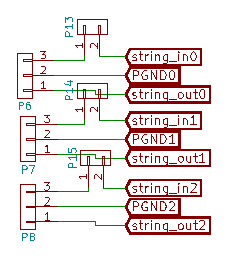
\includegraphics[width=\textwidth]{images/superv-sch/supervisor--sch--coupling.eps}
    \figcaption{Anschl\"usse zur Einkopplung}
    \label{fig:sch:master:coupling}
\end{minipage}}


% ---------------------------------------------------------------------------- %
\subsection{Strommessung}
\label{subsec:hw:master:current}
% ---------------------------------------------------------------------------- %


\begin{figure}[h!t]
    \centering
    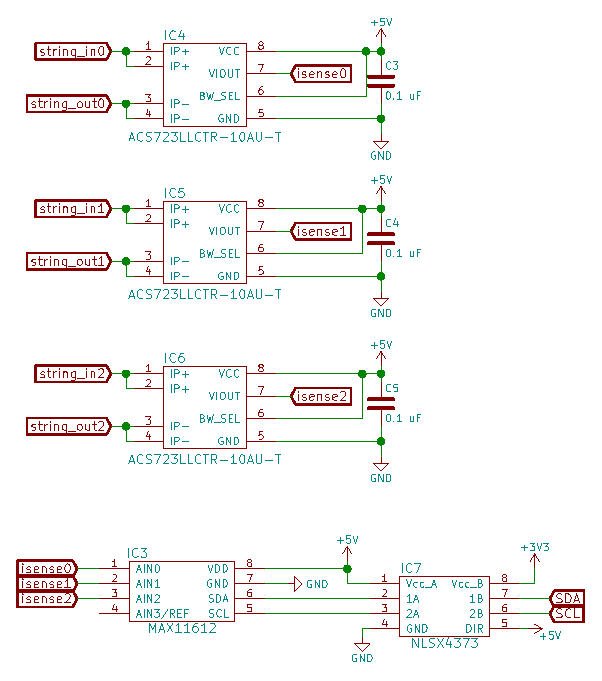
\includegraphics[width=0.75\textwidth]{images/superv-sch/supervisor--sch--current.eps}
    \caption{Strommessung}
    \label{fig:sch:master:current}
\end{figure}

\todo{Auswahl IC4, IC5, IC6, IC3, IC7, Gr\"osse C3, C4, C5}

Der  Strom jedes  Modulstrangs  wird separat  \"uberwacht;  die dazu  benutzte
Schaltung   ist   in   Abbildung   \ref{fig:sch:master:current}   dargestellt.
\code{IC4},  \code{IC5}  und  \code{IC6} sind  die  Strommessungssensoren. Sie
geben   auf   den    Leitungen   \code{isense0},   \code{isense1}   respektive
\code{isense2}   eine  Spannung   aus,  welche   dem  durch   sie  fliessenden
Strom  entspricht  (von  den  Modulen  in  die  Eing\"ange  \code{string\_in1}
usw.   geleitet,   anschliessend   via   \code{string\_out1}   usw.   an   den
Generatoranschlusskasten).

\code{IC3} ist der A/D-Konverter,  welcher die analogen Signale \code{isense0}
bis  \code{isense2}  in  digitale  Signale  mit  \SI{5}{\volt}-Pegel  wandelt.
\code{IC7} ist  ein Pegelwandler, welcher die  \SI{5}{\volt}-Signale auf einen
Pegel von  \SI{3.3}{\volt} konvertiert  f\"ur den Versand  via \ISC,  weil die
Eing\"ange des \Raspi~auf \SI{3.3}{\volt} laufen.

% ---------------------------------------------------------------------------- %
\clearpage
\subsection{GSM-Modem}
\label{subsec:hw:master:gsm}
% ---------------------------------------------------------------------------- %

\begin{figure}[h!t]
    \centering
    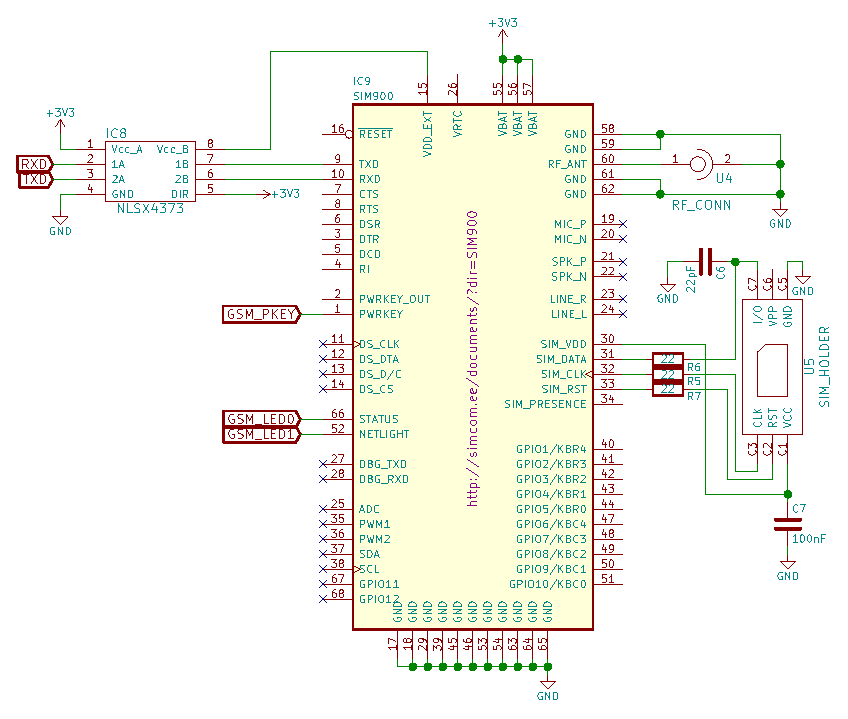
\includegraphics[width=0.85\textwidth]{images/superv-sch/supervisor--sch--gsm.eps}
    \caption{GSM-Modem Schaltung}
    \label{fig:sch:master:gsm}
\end{figure}

\todo{Auswahl IC8, Auswahl Modem, Gr\"osse C6, C7, R5, R6, R7}

Das GSM-Modem  ist ein  integrierter Baustein,  der alle  n\"otigen Funktionen
bereitstellt.    Er  ist   zusammen  mit   seiner  Beschaltung   in  Abbildung
\ref{fig:sch:master:gsm} dargestellt. Wie auch bei  der Strommessung wird auch
hier  ein  Pegelwandler  verwendet,  um  das Signal  von  der  UART-Linie  mit
\SI{3.3}{\volt} auf  den vom  GSM-Chip ben\"otigten Pegel  von \SI{2.8}{\volt}
(Pin  \code{VDD\_EXT}  auf  dem  Chip, verbunden  mit  \code{Vcc\_B}  auf  dem
Pegelwandler) zu wandeln.\todo{check values}

Der  Pin  \code{GSM\_PKEY} dient  zum  Einschalten  des GSM-Modems,  gesteuert
vom  \Raspi  via  GPIO  (siehe  Abschnitt  \ref{subsec:hw:master:gpio},  Seite
\pageref{subsec:hw:master:gpio}).

Via die beiden Pins \code{STATUS}  und \code{NETLIGHT} werden zwei Status-LEDs
angesteuert (siehe  ebenfalls Abschnitt  \ref{subsec:hw:master:gpio}). Auf der
rechten Seite des  Schaltungsblocks ist die Antenne und der  Adapter f\"ur die
SIM-Karte zu sehen.
